\documentclass[11pt]{article}

\usepackage[margin=1.1in]{geometry}
\usepackage{amsmath,amssymb,amsthm}
\usepackage{booktabs}
\usepackage{microtype}
\usepackage{xcolor}
\usepackage{tikz}
\usepackage{pgfplots}
\usepackage{caption}
\usepackage[hidelinks]{hyperref}

\pgfplotsset{compat=1.18}
\usetikzlibrary{arrows.meta,positioning,fit,backgrounds,calc,shapes.geometric}

% ---- palette -------------------------------------------------------------
\definecolor{rbred}{HTML}{B3202C}
\definecolor{rbblack}{HTML}{1A1A1A}
\definecolor{rbgrey}{HTML}{6E7278}
\definecolor{rblight}{HTML}{E8E6E1}
\definecolor{rbaccent}{HTML}{1F6F8B}

% ---- tikz styles ---------------------------------------------------------
\tikzset{
  ph/.style   = {rectangle, rounded corners=3pt, draw=rbgrey, thick,
                 fill=rblight, minimum height=8mm, minimum width=20mm,
                 font=\small\sffamily, align=center},
  st/.style   = {circle, draw=rbblack, thick, fill=white,
                 minimum size=7mm, font=\scriptsize, inner sep=1pt},
  term/.style = {rectangle, draw=rbred, thick, fill=rbred!8,
                 minimum size=6mm, font=\scriptsize, inner sep=2pt},
  ed/.style   = {-{Stealth[length=2mm]}, draw=rbgrey, thick},
  edr/.style  = {-{Stealth[length=2mm]}, draw=rbred, thick},
  lbl/.style  = {font=\scriptsize\sffamily, inner sep=1pt},
}

% ---- theorem environments ------------------------------------------------
\theoremstyle{plain}
\newtheorem{theorem}{Theorem}[section]
\newtheorem{lemma}[theorem]{Lemma}
\newtheorem{corollary}[theorem]{Corollary}
\theoremstyle{definition}
\newtheorem{definition}[theorem]{Definition}
\newtheorem{example}[theorem]{Example}
\theoremstyle{remark}
\newtheorem{remark}[theorem]{Remark}

% ---- notation ------------------------------------------------------------
\newcommand{\R}{\ensuremath{\mathsf{R}}}
\newcommand{\B}{\ensuremath{\mathsf{B}}}
\newcommand{\seat}[1]{\ensuremath{s_{#1}}}
\newcommand{\rlb}{\ensuremath{r_{\mathrm{lb}}}}
\newcommand{\blb}{\ensuremath{b_{\mathrm{lb}}}}
\newcommand{\Q}{\ensuremath{\mathcal{Q}}}
\newcommand{\Sig}{\ensuremath{\Sigma}}
\newcommand{\dtrans}{\ensuremath{\delta}}
\newcommand{\code}[1]{\texttt{\small #1}}

\title{\bfseries The Red/Black Game:\\[2pt]
       \large Rules, Deterministic Dynamics, and Exact State Enumeration\\[4pt]
       \normalsize (Heads-Up)}
\author{Noah Brauner}
\date{}

\begin{document}
\maketitle
\vspace{-3.2em}

\begin{abstract}
\noindent
Red/Black is a hidden-information bidding game played over a shared
$52$-card deck in which only color matters. This paper gives a complete
formal account of the two-player game as a \emph{deterministic, acyclic
finite transition system}: we specify the state set, input alphabet,
transition function, initial states and final states, and we count each of
them exactly. Three results organize the account. First, once the deal is
fixed the game is fully deterministic --- all chance is confined to the
initial state --- and the transition graph is acyclic, so every play
terminates in between $5$ and $9$ rounds. Second, the order in which cards
are flipped during a contest is irrelevant to the state, which collapses
procurement from a tree of flip sequences to a small lattice on two
counters. Third, the public projection of the state --- what an observer
knows --- reduces to two integers per seat, giving $6{,}051$ public
classes, of which exactly $5{,}485$ are reachable; the pruning is
concentrated almost entirely in one layer, where $59\%$ of the enumerable
classes cannot occur. We then characterize what that projection throws
away: it pins down the support of the public posterior exactly, but not its
shape, so two histories arriving at the same public state can leave an
observer with materially different beliefs. Every count in this paper is
machine-verified against the shipped rules engine. The paper is a precursor
to a companion paper on counterfactual regret minimization for the same
game.
\end{abstract}

\section{Introduction}

Red/Black is a bidding game for two to ten players. A shared $52$-card deck
is dealt face down; only the color of a card matters, and there are exactly
$26$ red and $26$ black. Players bid on how many cards of a chosen color
are in play across \emph{all} hands. An opponent either raises the bid or
challenges it, and a challenged bidder must literally produce the claimed
cards by flipping them, one at a time, off the top of any player's deck.
Fail, and you discard a card. Run out of cards and you are eliminated.

The game is small enough to be understood completely and large enough to be
interesting. This paper does the first half of that job: it describes the
game exactly, formalizes it as a finite transition system, and counts
everything. It deliberately says nothing about how to \emph{play} well.
Strategy, equilibrium and the algorithms that approximate it are the
subject of a companion paper; here we build the object those algorithms
will run on.

\paragraph{Scope.} We restrict throughout to the \textbf{heads-up} ($N=2$)
game. The rules in Section~\ref{sec:rules} are stated for two players; where
a rule generalizes awkwardly we say so. All counting is heads-up.

\paragraph{Contributions.}
\begin{enumerate}\itemsep2pt
  \item A complete formal specification of Red/Black as a deterministic
        transition system, with an explicit account of where the
        randomness lives and what the automaton does \emph{not} capture
        (Section~\ref{sec:automaton}).
  \item Termination and acyclicity theorems: the heads-up game lasts
        between $5$ and $9$ rounds, and no state is ever revisited
        (Theorems~\ref{thm:acyclic} and~\ref{thm:rounds}).
  \item An order-irrelevance lemma for procurement
        (Lemma~\ref{lem:order}) that collapses the contest phase from a
        tree of flip sequences to a lattice on two counters, and the exact
        node counts that follow (Section~\ref{sec:round}).
  \item Exact enumeration of the public state space: a closed form
        $\binom{H+3}{3}-1$ for the per-seat public statistic, hence
        $6{,}051$ public classes at hand size $H=5$
        (Section~\ref{sec:full}).
  \item An exact reachability closure showing only $5{,}485$ of those
        $6{,}051$ classes can occur, with the obstruction identified and
        proved (Section~\ref{sec:reach}).
  \item A characterization of what the public state \emph{omits}: the
        bounds describe the support of the public posterior exactly
        (Theorem~\ref{thm:support}) but not its shape, and two histories
        reaching the same class can leave an observer with materially
        different beliefs (Section~\ref{sec:forgets}).
\end{enumerate}

\paragraph{Reproducibility.}
Every numeral in this paper is produced by \code{state\_counts.py}, which
re-derives the combinatorics from the rules independently of the game
engine, and cross-checked against the shipped engine by
\code{verify\_against\_engine.py}. Both accompany this document.

\paragraph{Road map.} Section~\ref{sec:rules} states the rules.
Section~\ref{sec:automaton} builds the automaton. We then climb a ladder of
three games, identical in rules and differing only in how many cards each
player is dealt: the one-card game (Section~\ref{sec:h1}), small enough to
draw in full; the two-card game (Section~\ref{sec:h2}), the smallest game
with a real bidding ladder and a real discard choice; and the actual
five-card game (Section~\ref{sec:full}). Section~\ref{sec:reach} settles
reachability, Section~\ref{sec:forgets} examines what the public state
deliberately throws away, and Section~\ref{sec:next} hands off to the
companion paper.

\paragraph{Notation.} Symbols are fixed for the whole paper and collected
in Table~\ref{tab:notation}. Seats are always $0$ and $1$, and $i$ always
ranges over them. Two conventions prevent collisions: lower bounds always
carry the $\mathrm{lb}$ subscript, so $b_i$ (blacks held) is never confused
with $\blb^{\,i}$ (blacks known to be held); and bid counts are written $k$
or $\kappa$, never $b$. A primed symbol always means ``after the pending
discard'' --- the distinction is the subject of Section~\ref{sec:twoclocks},
and it is the one place where the rules' ordering and the analysis' ordering
disagree.

\begin{table}[htbp]
\centering
\caption{Notation used throughout.}
\label{tab:notation}
\small
\begin{tabular}{@{}llc@{}}
\toprule
Symbol & Meaning & Defined \\
\midrule
$N$ & number of players; $N=2$ throughout & \S\ref{sec:rules}\\
$H$ & hand size at the deal, and the most a seat can ever hold & \S\ref{sec:rules}\\
$n_i$ & cards in seat $i$'s hand \emph{now} (at a boundary: pre-discard) & Def.~\ref{def:state}\\
$T$ & cards in play now, $T=n_0+n_1$ & Def.~\ref{def:state}\\
$n_i'$ & seat $i$'s hand size \emph{during} the next round (post-discard) & \S\ref{sec:twoclocks}\\
$T'$ & cards in play during the next round; the \textbf{layer index} & \S\ref{sec:twoclocks}\\
$r_i,\;b_i$ & reds and blacks currently in seat $i$'s hand, $r_i+b_i=n_i$ & \S\ref{sec:closure}\\
$\rho$ & phase & Def.~\ref{def:state}\\
$\sigma$ & seat that starts the current round & Def.~\ref{def:state}\\
$h_i$ & seat $i$'s hand as an \emph{ordered} tuple of colors & Def.~\ref{def:state}\\
$\beta$ & bid history: a color plus a chain $k_1<\dots<k_m$ & Def.~\ref{def:state}\\
$\nu,\;\lambda$ & the bidder; the loser of the contest just resolved & Def.~\ref{def:state}\\
$\varphi_i$ & cards flipped off seat $i$'s deck this contest & Def.~\ref{def:state}\\
$c$ & the bid color of the current round & \S\ref{sec:rules}\\
$k,\;\kappa$ & a bid count; the \emph{final} count of a chain ($\kappa=k_m$) & \S\ref{sec:rules}\\
$x,\;y$ & flips taken off the bidder's / the challenger's deck & Lem.~\ref{lem:proccount}\\
$L$ & lattice-point count for procurement & Lem.~\ref{lem:proccount}\\
$\ell$ & seat owing a discard at a boundary; $-1$ at the root & Def.~\ref{def:class}\\
$s_i$ & seat $i$'s public statistic $(n_i,\rlb^{\,i},\blb^{\,i})$ & Def.~\ref{def:class}\\
$\rlb^{\,i},\;\blb^{\,i}$ & certainty bounds: reds / blacks seat $i$ surely holds & Def.~\ref{def:class}\\
$K(H)$ & number of distinct per-seat public statistics & Thm.~\ref{thm:seatcount}\\
$m_i,\;e_i$ & on-color / off-color cards revealed from seat $i$ in a round & Lem.~\ref{lem:sighting}\\
\bottomrule
\end{tabular}
\end{table}

% =========================================================================
\section{The Rules}\label{sec:rules}

\subsection{Components and setup}

One shared deck of $52$ cards, exactly $26$ \textcolor{rbred}{red} and $26$
\textcolor{rbblack}{black}. Suits and ranks do not exist: a card's only
attribute is its color. Each of the two players is dealt $H=5$ cards; the
remaining $52-2H=42$ cards are removed from the game and never seen by
anyone. Hands only ever shrink --- no card is drawn after the deal.

A player's hand is an \emph{ordered} list. Index $0$ is the top of the
deck: the first card that will be flipped if someone procures from it.
Players see their own cards and nothing of their opponent's except its
size, which is always public.

\subsection{A round}

A round has four phases, in order.

\begin{enumerate}\itemsep3pt
  \item[\textbf{1.}] \textbf{Reorder.} Both players privately and
        simultaneously rearrange their own hand and confirm. This is the
        only moment hand order can change.
  \item[\textbf{2.}] \textbf{Bidding.} The starting player bids a pair
        $(k,c)$: a count $k\ge 1$ and a color $c$, claiming that at least
        $k$ cards of color $c$ are in play across both hands. The count is
        capped by the total number of cards in play. Thereafter players
        alternate, and each must do exactly one of:
        \emph{raise} (same color, strictly greater count) or
        \emph{challenge}. The color is fixed by the first bid and never
        changes within a round. Passing is not a legal move.
  \item[\textbf{3.}] \textbf{Procurement.} A challenge ends bidding. The
        last bidder must now produce the claim. They repeatedly flip the
        top card of \emph{either} player's deck --- their own or the
        opponent's, switching freely --- and each flipped color is
        revealed publicly. The first off-color flip is fatal: the bidder
        loses immediately. Reaching the claimed count of on-color cards
        wins: the challenger loses.
  \item[\textbf{4.}] \textbf{Discard.} The loser of the contest secretly
        removes one card from their hand. The identity of that card is
        never revealed. If the loser holds exactly one card, the discard is
        forced and eliminates them.
\end{enumerate}

The winner of the contest starts the next round. In round~1 the starting
player is seat~$0$. A player with zero cards is eliminated and the other
player wins.

\begin{figure}[t]
\centering
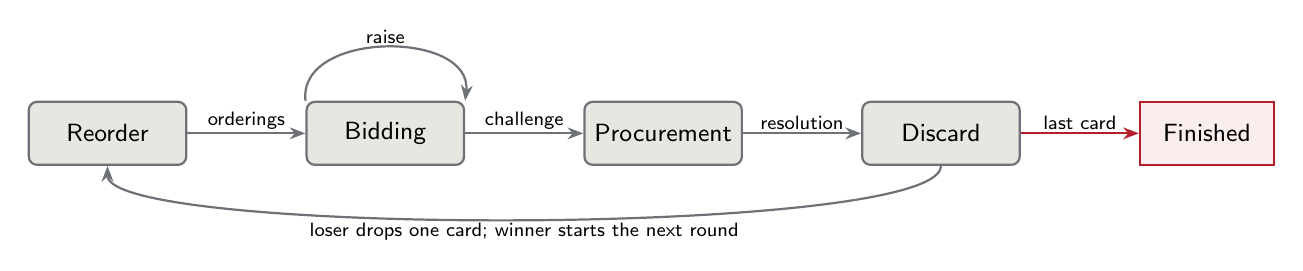
\begin{tikzpicture}[node distance=8mm and 15mm]
  \node[ph] (reo) {Reorder};
  \node[ph, right=of reo] (bid) {Bidding};
  \node[ph, right=of bid] (pro) {Procurement};
  \node[ph, right=of pro] (dis) {Discard};
  \node[term, right=of dis, minimum height=8mm, minimum width=17mm,
        font=\small\sffamily] (fin) {Finished};
  \draw[ed] (reo) -- node[lbl,above]{orderings} (bid);
  \draw[ed] (bid) -- node[lbl,above]{challenge} (pro);
  \draw[ed] (pro) -- node[lbl,above,align=center]{resolution} (dis);
  \draw[edr] (dis) -- node[lbl,above,align=center]{last card} (fin);
  \draw[ed] (dis.south) .. controls +(0,-9mm) and +(0,-9mm) ..
        node[lbl,below]{loser drops one card; winner starts the next round} (reo.south);
  \draw[ed] (bid.north west) .. controls +(-1mm,9mm) and +(1mm,9mm) ..
        node[lbl,above]{raise} (bid.north east);
\end{tikzpicture}
\caption{The four phases of a round. The only cycle in the \emph{phase}
graph is the round loop; it is not a cycle in the state graph, because one
card leaves play on every pass (Theorem~\ref{thm:acyclic}).}
\label{fig:phases}
\end{figure}

\subsection{Information}\label{sec:info}

What is public at all times: both hand sizes, whose turn it is, the current
round's full bid history, and the full flip history of the current contest.
What is private: the colors and order of your own hand, and the identity
of any card you yourself discarded.

Two rules do most of the work in this paper.

\begin{description}\itemsep3pt
  \item[Discard anonymity.] The discarded card's identity is never
        revealed. Observers learn only that a hand shrank by one.
  \item[Reorder scrambling.] Cards flipped in round $k$ are identifiable
        only within round $k$. Once the next reorder happens, all of a
        player's cards are anonymous card backs again.
\end{description}

Together these mean no \emph{card identity} survives a round boundary. What
survives is strictly weaker: multiset knowledge, degraded by discards. If
you saw two reds flipped from my hand, you know I hold at least two reds
--- until I discard, at which point you know only that I hold at least one,
because the card I dropped may have been one of them. We make this precise
in Section~\ref{sec:public}.

% =========================================================================
\section{The Game as a Deterministic Transition System}\label{sec:automaton}

\subsection{Is it a finite state machine?}

Yes, with one clarification worth making carefully, because the phrase
``hidden information'' suggests otherwise.

A deterministic finite automaton is a tuple $(\Q,\Sig,\dtrans,q_0,F)$ with
$\dtrans:\Q\times\Sig\to\Q$ a \emph{function} --- one input, one successor,
no coin flips. Red/Black satisfies this once we are careful about two
things:

\begin{enumerate}\itemsep2pt
  \item \textbf{The randomness is in the initial state, not the
        transitions.} The deal is the only chance event in the entire game.
        Fix it, and every subsequent transition is a deterministic function
        of the current state and the acting player's move. So Red/Black is
        a \emph{family} of deterministic automata indexed by the deal, or
        equivalently one automaton whose first input letter is the deal.
  \item \textbf{Hidden information is a property of the observers, not of
        the machine.} The state is perfectly well defined at all times; it
        is simply that neither player can see all of it. Formally, hidden
        information is an \emph{equivalence relation on $\Q$}
        (Section~\ref{sec:partition}), layered on top of a machine that is
        itself deterministic.
\end{enumerate}

So the intuition is right. The machine is deterministic. What a finite
state machine does not by itself express is who can distinguish which
states --- and that is exactly the structure the companion paper needs.

\subsection{The state}

\begin{definition}[Game state]\label{def:state}
A state is a tuple
\[
  q \;=\; \bigl(\rho,\; \sigma,\; h_0,\; h_1,\; \beta,\; \nu,\;
                 \varphi_0,\; \varphi_1,\; \lambda \bigr)
\]
with components
\begin{center}
\begin{tabular}{@{}ll@{}}
\toprule
$\rho$ & phase, $\rho\in\{\textsc{reorder},\textsc{bid},\textsc{proc},\textsc{disc},\textsc{fin}\}$\\
$\sigma$ & starting seat of the current round, $\sigma\in\{0,1\}$\\
$h_i$ & seat $i$'s hand: an ordered tuple of colors, $h_i\in\{\R,\B\}^{n_i}$\\
$\beta$ & bid history: $\bot$, or a pair $(c,\,k_1<\dots<k_m)$ of a color and a chain of counts\\
$\nu$ & the bidder (last raiser) once a challenge has occurred, else $\bot$\\
$\varphi_i$ & cards already flipped from seat $i$'s deck this contest\\
$\lambda$ & the loser of the contest just resolved, else $\bot$\\
\bottomrule
\end{tabular}
\end{center}
We write $n_i=|h_i|$ for hand sizes and $T=n_0+n_1$ for the total cards in
play.
\end{definition}

\begin{remark}[What is deliberately absent]\label{rem:absent}
The state carries no record of \emph{which} cards have been discarded, nor
of past rounds' bids or flips. Neither affects any player's legal moves or
any future transition: discarded cards are gone from play, and a past
round's bid history is cleared. They affect only what the players
\emph{believe}, which is the subject of Section~\ref{sec:partition} and of
the companion paper. Keeping them out of $\Q$ is what makes the state space
finite and small.
\end{remark}

\subsection{The input alphabet}

\begin{definition}[Inputs]\label{def:inputs}
$\Sig=\Sig_{\mathrm{deal}}\cup\Sig_{\mathrm{ord}}\cup\Sig_{\mathrm{bid}}
       \cup\Sig_{\mathrm{proc}}\cup\Sig_{\mathrm{disc}}$, where
\begin{center}\small
\begin{tabular}{@{}llr@{}}
\toprule
Phase & Letters available & How many\\
\midrule
--- & $\code{deal}(D)$, a split of $2H$ cards & $\binom{52}{H}\binom{52-H}{H}$ \\
\textsc{reorder} & $\code{order}(\pi)$, an ordering of one's own hand & $\binom{n_i}{r_i}$ per seat\\
\textsc{bid} & $\code{bid}(c,k)$, $c\in\{\R,\B\}$, $1\le k\le T$ & $2T$\\
\textsc{bid} & $\code{raise}(k)$, $k$ above the current count & $\le T-1$\\
\textsc{bid} & $\code{challenge}$ & $1$\\
\textsc{proc} & $\code{flip}(j)$, $j$ the target seat & $\le 2$\\
\textsc{disc} & $\code{drop}(c)$, $c\in\{\R,\B\}$ & $\le 2$\\
\bottomrule
\end{tabular}
\end{center}
Opening bids and raises are mutually exclusive: \code{bid} is legal only on
an empty history, \code{raise} and \code{challenge} only on a non-empty one.
\end{definition}

$\dtrans$ is a \emph{partial} function: illegal letters have no successor.
One may complete it in the usual way with an absorbing dead state; we leave
it partial, since the legal-move set is itself part of the game's
description.

\subsection{Initial and final states}

\begin{definition}[Initial states]
$q_0$ is the pre-deal state. After the single chance letter
$\code{deal}(D)$ the machine occupies
$\bigl(\textsc{reorder},\,0,\,h_0,\,h_1,\,\bot,\,\bot,\,0,\,0,\,\bot\bigr)$
with $|h_0|=|h_1|=H$. Seat $0$ starts round $1$ by convention.
\end{definition}

\begin{definition}[Final states]
$F$ is the set of states with $\rho=\textsc{fin}$, equivalently those in
which some $n_i=0$. The other player is the winner. There are no draws:
exactly one player is eliminated, and the game ends the moment that
happens.
\end{definition}

\subsection{Determinism, acyclicity, termination}

\begin{theorem}[Determinism]\label{thm:det}
For every state $q$ and every legal letter $a$, the successor
$\dtrans(q,a)$ is uniquely determined. No transition consults a random
source.
\end{theorem}

\begin{proof}
Inspect each phase. \textsc{reorder} replaces $h_i$ by a stated
permutation. \textsc{bid} appends to $\beta$ or moves to \textsc{proc} and
records $\nu$. In \textsc{proc}, the letter names a target seat $j$; the
card revealed is $h_j[\varphi_j]$, already fixed in the state, and the
outcome is a comparison of that color against $\beta$'s color: off-color
$\Rightarrow$ bidder loses, else increment $\varphi_j$ and check the count.
\textsc{disc} names a color and removes one such card. In every case the
successor is a function of $(q,a)$ alone.
\end{proof}

The subtle point is in \textsc{proc}: the flipped card looks random to the
players, but it is not random to the machine. It was fixed at the deal and
positioned at the last reorder. Uncertainty here is epistemic, not
stochastic.

\begin{theorem}[Acyclicity]\label{thm:acyclic}
The transition graph is acyclic.
\end{theorem}

\begin{proof}
Take the lexicographic rank $\Phi(q)=\bigl(T,\;-|\beta|,\;
-(\varphi_0+\varphi_1)\bigr)$ ordered so that every transition strictly
decreases it. Within a contest, each \code{flip} increments
$\varphi_0+\varphi_1$ and leaves $T$ and $|\beta|$ fixed. Within bidding,
each \code{bid} or \code{raise} increments $|\beta|$ and leaves $T$ fixed;
\code{challenge} moves to \textsc{proc} with $\varphi_0+\varphi_1=0$, which
is handled by treating phase order as a tiebreak. Each \code{drop}
decrements $T$ by exactly one, resetting the later components. As $T$
strictly decreases once per round and never increases, no state recurs.
\end{proof}

\begin{theorem}[Round bounds]\label{thm:rounds}
The heads-up game with hand size $H$ lasts at least $H$ and at most $2H-1$
rounds. For the real game ($H=5$) that is between $5$ and $9$ rounds.
\end{theorem}

\begin{proof}
Exactly one card leaves play per round, and a seat is eliminated on its
$H$-th discard. The minimum is achieved when the same seat loses every
round: $H$ rounds. For the maximum, the game is still alive after $k$
rounds only if both seats have made at most $H-1$ discards, so
$k\le 2(H-1)$; the game therefore ends on round $2H-1$ at the latest, and
that bound is achieved by alternating losses.
\end{proof}

\begin{corollary}\label{cor:counter}
Total cards in play is a strictly decreasing round counter running
$2H,\,2H-1,\,\dots$ down to the terminal value, so it is a natural index for
induction over the game. Section~\ref{sec:twoclocks} fixes precisely which
version of that count we index by --- the one measured \emph{during} a
round rather than at its boundary --- and calls it $T'$.
\end{corollary}

\subsection{What the automaton omits: the information partition}
\label{sec:partition}

\begin{definition}[Observation and indistinguishability]
Let $\mathrm{obs}_i(q)$ be the part of $q$ visible to seat $i$: the phase,
the starter, both hand sizes, the current bid history $\beta$, the flip
counters and the colors revealed so far this contest, plus seat $i$'s own
hand $h_i$. Write $q\sim_i q'$ when $\mathrm{obs}_i(q)=\mathrm{obs}_i(q')$.
The classes of $\sim_i$ are seat $i$'s \emph{information sets}.
\end{definition}

$\sim_i$ is what makes Red/Black a game rather than a puzzle, and it is
invisible to $(\Q,\Sig,\dtrans,q_0,F)$. Two facts about it matter here:

\begin{enumerate}\itemsep2pt
  \item \textbf{Perfect recall} holds: a player never forgets their own
        past observations or moves. This is what licenses the algorithms of
        the companion paper.
  \item \textbf{The public projection}, $\mathrm{pub}(q)$ --- everything
        both players see --- is far smaller than $q$, and at round
        boundaries it collapses to just four integers.
        Section~\ref{sec:public} derives it, and it is the object the whole
        second half of this paper counts.
\end{enumerate}

% =========================================================================
\section{The Round Automaton}\label{sec:round}

Before climbing the ladder of games we isolate the structure of a
\emph{single} round, which is independent of the deal and depends only on
the starter $\sigma$ and the hand sizes $(n_0,n_1)$.

\subsection{Bidding}

A bid history is a color together with a strictly increasing chain of
counts drawn from $\{1,\dots,T\}$. Chains are in bijection with non-empty
subsets of $\{1,\dots,T\}$.

\begin{lemma}[Bid node count]\label{lem:bidcount}
The number of bidding states with $T$ cards in play is
\[
  1 \;+\; 2\left(2^{T}-1\right) \;=\; 2^{\,T+1}-1 .
\]
\end{lemma}

\begin{proof}
One pre-bid state; then a state per (color, non-empty chain) pair, and
there are $2^T-1$ non-empty subsets of $\{1,\dots,T\}$ and two colors.
\end{proof}

So $T=2$ gives $7$ states, $T=4$ gives $31$, and the full game's opening
round ($T=10$) gives $2{,}047$. The seat to act at a chain of length $m$ is
$\sigma$ if $m$ is even and $1-\sigma$ otherwise; the bidder --- the seat
that will have to produce the claim --- is whoever placed the last bid.

\begin{remark}[A constraint we will need]\label{rem:ladder}
Because the starter bids first and counts strictly increase, a
\emph{non-starter} can only be the bidder if at least two bids were placed,
which forces the final count to be at least $2$. A final count of $1$ pins
the bidder to be the starter. This small fact prunes real states in
Section~\ref{sec:reach}.
\end{remark}

\subsection{Procurement, and why order does not matter}

\begin{lemma}[Order irrelevance]\label{lem:order}
During a contest, the state depends only on the pair of counters
$(\varphi_0,\varphi_1)$ and not on the order in which the flips were made.
\end{lemma}

\begin{proof}
A contest continues only while every flipped card has matched the bid
color. Hence at any live procurement state, the multiset of revealed cards
is determined: $\varphi_0+\varphi_1$ cards, all of the bid color, of which
$\varphi_i$ came off seat $i$'s deck. Each deck is consumed strictly top
down, so which cards remain is likewise determined by the counters alone.
Two flip sequences with the same counters therefore yield identical states.
\end{proof}

Lemma~\ref{lem:order} is what makes the game tractable: procurement is a
\emph{lattice} on two counters, not a tree of flip sequences. A naive
sequence count at $T=10$ would be exponential in the number of flips; the
lattice is quadratic.

A second, independent collapse applies to the \emph{orderings} themselves.

\begin{lemma}[Hand orderings collapse at the first color change]
\label{lem:orderclass}
Let a seat's post-reorder hand open with a maximal run of color $a$ of
length $k$. Then nothing at position $k+2$ or beyond can ever be revealed,
under either bid color. Consequently two orderings are strategically
indistinguishable whenever they agree on the pair
\[
  (a,\;k)\;=\;(\text{leading color},\;\text{leading run length}),
\]
and the number of distinguishable orderings of an $(r,\,b)$ multiset is
\[
  F(r,b)\;=\;
  \begin{cases}
    1, & r=0 \text{ or } b=0,\\
    r+b, & \text{otherwise,}
  \end{cases}
\]
against $\binom{r+b}{r}$ raw orderings.
\end{lemma}

\begin{proof}
Procurement from a seat's deck consumes cards top down and stops at that
seat's first off-color card. If the bid color is $a$, the flips take the $k$
cards of the leading run and then the card at $k+1$, which is $\neg a$ by
maximality, and which is fatal. If the bid color is $\neg a$, the very first
flip is off-color and fatal. In both cases consumption halts at position
$k+1$ at the latest, so positions $k+2,\dots,n$ are never seen.

Nor can they matter later. Flipping does not remove a card
(Section~\ref{sec:rules}), so a round leaves hand \emph{composition}
untouched; and every round begins with a fresh reorder, so no ordering
survives a boundary. Hence the tail is unobservable and irrelevant, and the
observable content of an ordering is exactly $(a,k)$.

For the count: with both colors present, the leading run may be $a=$~red of
length $1..r$ or $a=$~black of length $1..b$, giving $r+b$ classes; a
single-color hand admits one.
\end{proof}

\begin{remark}[Size of the collapse]\label{rem:ordersave}
The saving needs $n\ge 4$ to appear at all --- for $n\le 3$,
$\binom{n}{r}=F$ exactly --- and is capped at $50\%$ per composition
($\binom{5}{2}=10\to 5$). Balanced hands save; lopsided ones
($r\in\{0,1,n-1,n\}$) save nothing. Summed over every reachable private
state of the full game the reduction is $12\%$
($172{,}488\to 150{,}964$), but it is worth more than that in practice
because it grows with depth --- $0\%$ at $T'\le 4$, $15\%$ at $T'=8$,
$24\%$ at $T'=9$, $31\%$ at the root --- and the deep layers hold most of
the work. Weighted by how many decisions actually sit in each layer it is
about $19\%$; the companion paper tabulates those weights.

Note this is a \emph{lossless} collapse, like Lemma~\ref{lem:order} and
unlike the belief abstraction of Section~\ref{sec:forgets}: merged
orderings are indistinguishable in every continuation, so nothing is
approximated.
\end{remark}

\begin{lemma}[Procurement node count]\label{lem:proccount}
Fix a color and a chain $k_1<\dots<k_m$, and write $n_{\mathrm{bid}}$ and
$n_{\mathrm{chal}}$ for the hand sizes of the bidder and the challenger.
The live procurement states for that chain number
\[
  L\bigl(k_m-1,\;n_{\mathrm{bid}},\;n_{\mathrm{chal}}\bigr)\;=\;
  \#\bigl\{(x,y)\in\mathbb{Z}_{\ge0}^2 \;:\; x+y\le k_m-1,\;
        x\le n_{\mathrm{bid}},\; y\le n_{\mathrm{chal}}\bigr\},
\]
where $x$ and $y$ count the cards already flipped off the bidder's and the
challenger's decks respectively. Summing over both colors and all
$2^{\,k_m-1}$ chains with final count $k_m$ gives the round's total. When
$n_0=n_1=n$ this is
\[
  \#\textsc{proc}(T,n)\;=\;2\sum_{\kappa=1}^{T}2^{\,\kappa-1}\,L(\kappa-1,n,n),
\]
the sum running over the possible final counts $\kappa$.
\end{lemma}

The constraint $x+y\le k_m-1$ is the statement that the bid is not yet
made: at $x+y=k_m$ the bidder has produced the claim and the round is over.

\begin{figure}[t]
\centering
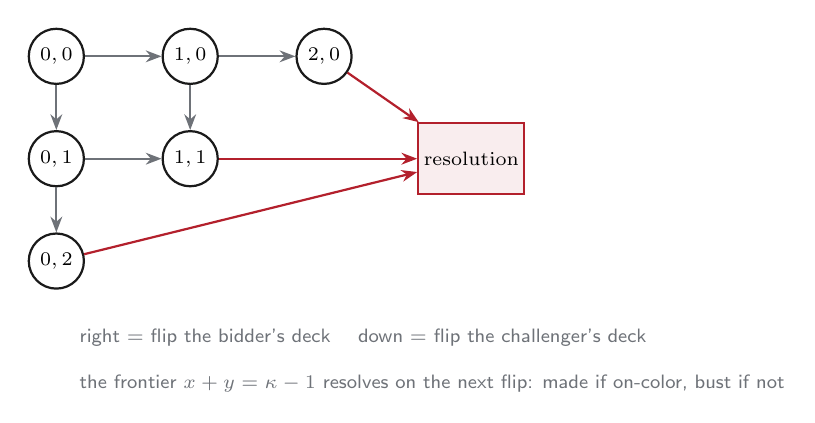
\begin{tikzpicture}[x=17mm,y=-13mm]
  \foreach \x/\y in {0/0, 1/0, 2/0, 0/1, 1/1, 0/2}{
    \node[st] (n\x\y) at (\x,\y) {$\x,\y$};
  }
  \foreach \a/\b in {00/10, 10/20, 01/11, 00/01, 10/11, 01/02}{
    \draw[ed] (n\a) -- (n\b);
  }
  \node[term, minimum height=9mm] (res) at (3.1,1) {resolution};
  \foreach \n in {n20, n11, n02}{ \draw[edr] (\n) -- (res); }
  \node[lbl, anchor=west, text=rbgrey] at (0.15,2.75)
    {right $=$ flip the bidder's deck \quad down $=$ flip the challenger's deck};
  \node[lbl, anchor=west, text=rbgrey] at (0.15,3.2)
    {the frontier $x+y=\kappa-1$ resolves on the next flip: made if on-color, bust if not};
\end{tikzpicture}
\caption{The procurement lattice for a final bid count of $\kappa=3$ with
two cards in each hand. A state is the pair $(x,y)$ counting cards already
flipped off the bidder's and the challenger's decks; by
Lemma~\ref{lem:order} the path taken to a node is irrelevant. Only the
$x+y\le \kappa-1=2$ nodes are live.}
\label{fig:proclattice}
\end{figure}

\subsection{Resolutions}

Every contest ends in one of two ways, and the resolution records enough to
continue the game: the color and chain, the final counters, whether the
loser was the bidder, and --- when the bidder busted --- which deck the
fatal card came off. That last datum matters because it tells observers
whose hand certainly contains an off-color card.

Table~\ref{tab:round} collects the three counts for the hand-size
configurations used later.

\begin{table}[t]
\centering
\caption{The round automaton, per $(n_0,n_1)$. Counts are independent of the
starter, and every entry is verified against the shipped graph builder.}
\label{tab:round}
\begin{tabular}{@{}lrrrr@{}}
\toprule
Configuration & $T$ & Bid states & Procurement states & Resolutions\\
\midrule
$(1,1)$ \quad one-card game & $2$  & $7$     & $14$     & $28$\\
$(2,2)$ \quad two-card game & $4$  & $31$    & $190$    & $348$\\
$(5,5)$ \quad opening round & $10$ & $2{,}047$ & $65{,}790$ & $119{,}036$\\
$(3,5)$ \quad a later round & $8$  & $511$   & $10{,}398$ & $18{,}588$\\
\bottomrule
\end{tabular}
\end{table}

% =========================================================================
\section{The Public State at a Round Boundary}\label{sec:public}

We now derive the projection $\mathrm{pub}(q)$ that both players share. It
is the single most useful object in the paper.

\subsection{What survives a round}

Fix the moment a contest resolves: the loser is known, but has not yet
discarded. Call this a \emph{boundary}. By the rules of
Section~\ref{sec:info}, an observer at a boundary knows: both hand sizes,
who lost, and --- from the flips just seen, plus memory of earlier rounds
--- a lower bound on how many cards of each color each seat certainly
still holds. Nothing else about cards survives, because discard anonymity
and reorder scrambling destroy identity.

\begin{definition}[Public class]\label{def:class}
A boundary's public state is
\[
  \bigl(\ell,\; \seat{0},\; \seat{1}\bigr),\qquad
  \seat{i}=\bigl(n_i,\;\rlb^{\,i},\;\blb^{\,i}\bigr),
\]
where $\ell\in\{-1,0,1\}$ names the seat that owes a discard ($-1$ at the
game root), $n_i$ is seat $i$'s hand size \emph{before} that discard, and
$\rlb^{\,i},\blb^{\,i}$ are the certainty bounds: everyone knows seat $i$
holds at least $\rlb^{\,i}$ reds and at least $\blb^{\,i}$ blacks. The next
round's starter is $1-\ell$, so it need not be stored.
\end{definition}

\begin{lemma}[Bound folding]\label{lem:fold}
Across a round, the bounds evolve as
\[
  \rlb \;\longmapsto\; \max\bigl(\,\rlb-[\,\text{this seat discarded}\,],\;
                        \#\{\text{reds seen from this seat this round}\}\,\bigr),
\]
and symmetrically for $\blb$. The fold is a maximum, never a sum.
\end{lemma}

\begin{proof}
A discard removes an unknown card, so a bound of $\rlb$ degrades to
$\rlb-1$ (floored at zero): the dropped card may have been one of the
counted reds. Cards flipped this round are certainly still held, giving a
fresh bound. The two cannot be added, because a red seen this round may be
one of the reds already counted; only the larger is certain.
\end{proof}

\begin{lemma}[Certainty is bounded by holdings]\label{lem:cap}
$\rlb^{\,i}+\blb^{\,i}\le n_i$ at every boundary.
\end{lemma}

\subsection{Two clocks: where the discard sits}\label{sec:twoclocks}

There is one genuine offset in this paper, and it causes trouble if left
implicit, so we make it explicit here and use it consistently afterwards.

\textbf{The rules order a round as} reorder $\to$ bidding $\to$ procurement
$\to$ \emph{discard}: the discard is the \emph{last} thing that happens
(Section~\ref{sec:rules}, Figure~\ref{fig:phases}). That is the right
description of the game as played.

\textbf{But the natural place to cut the game is not the same place.} We cut
at a \emph{boundary} --- a procurement resolution, where the loser is known
but has not yet discarded --- because that is the moment at which the public
state is a clean summary. Cutting there means the segment between two
consecutive boundaries reads \emph{discard} $\to$ reorder $\to$ bidding
$\to$ procurement: the discard is now the \emph{first} thing that happens.

Nothing about the game changed. The same events occur in the same order;
only the cut points moved, by exactly one discard.

\begin{figure}[htbp]
\centering
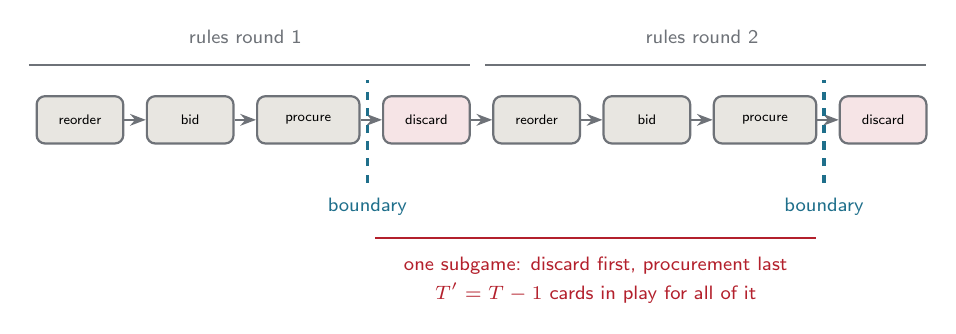
\begin{tikzpicture}[x=1mm,y=1mm]
  % --- event tape
  \foreach \k/\off in {1/0, 2/58}{
    \node[ph, minimum width=11mm, minimum height=6mm, font=\tiny\sffamily]
      (reo\k) at (\off+7,0) {reorder};
    \node[ph, minimum width=11mm, minimum height=6mm, font=\tiny\sffamily]
      (bid\k) at (\off+21,0) {bid};
    \node[ph, minimum width=13mm, minimum height=6mm, font=\tiny\sffamily]
      (pro\k) at (\off+36,0) {procure};
    \node[ph, minimum width=11mm, minimum height=6mm, fill=rbred!12,
          font=\tiny\sffamily] (dis\k) at (\off+51,0) {discard};
  }
  \draw[ed] (reo1)--(bid1); \draw[ed] (bid1)--(pro1); \draw[ed] (pro1)--(dis1);
  \draw[ed] (dis1)--(reo2); \draw[ed] (reo2)--(bid2); \draw[ed] (bid2)--(pro2);
  \draw[ed] (pro2)--(dis2);

  % --- rules brackets (above)
  \draw[decorate, draw=rbgrey, thick] (0.5,7) -- (56.5,7);
  \node[lbl, text=rbgrey] at (28,10.5) {rules round 1};
  \draw[decorate, draw=rbgrey, thick] (58.5,7) -- (114.5,7);
  \node[lbl, text=rbgrey] at (86,10.5) {rules round 2};

  % --- boundary markers
  \foreach \x in {43.5, 101.5}{
    \draw[rbaccent, very thick, dashed] (\x,-8) -- (\x,5);
  }
  \node[lbl, text=rbaccent] at (43.5,-11) {boundary};
  \node[lbl, text=rbaccent] at (101.5,-11) {boundary};

  % --- subgame bracket (below)
  \draw[decorate, draw=rbred, thick] (44.5,-15) -- (100.5,-15);
  \node[lbl, text=rbred] at (72.5,-18.5)
    {one subgame: discard first, procurement last};
  \node[lbl, text=rbred] at (72.5,-22)
    {$T'=T-1$ cards in play for all of it};
\end{tikzpicture}
\caption{The same event tape, cut two ways. The rules bracket a round from
reorder to discard (grey, above). The analysis brackets a subgame from one
procurement resolution to the next (red, below), so the discard moves to the
front. A boundary sits between procurement and discard, which is why a
boundary's hand sizes $n_i$ are \emph{pre}-discard while the round that
follows is played with $n_i'$.}
\label{fig:twoclocks}
\end{figure}

\begin{definition}[In-round sizes and the layer index]\label{def:layer}
At a boundary with pending discarder $\ell$, write
\[
  n_i' \;=\; n_i - [\,i=\ell\,],
  \qquad
  T' \;=\; n_0'+n_1' \;=\; T - [\,\ell\ge 0\,].
\]
So $n_i$ and $T$ describe the table at the boundary; $n_i'$ and $T'$
describe it for the entire round that follows, since no card leaves play
between the discard and the next resolution. We index classes by $T'$, the
\textbf{layer}.
\end{definition}

\begin{remark}[Why the layer is $T'$ and not $T$]
Two boundaries with the same $T$ can have different amounts of play left:
the game root has $T=10$ with no discard pending, whereas a resolution at
$n_0=n_1=5$ also has $T=10$ but owes a discard, so only $9$ cards will
actually be bid over. Indexing by $T'$ puts them in different layers, which
is what makes the class space a clean DAG with exactly one edge per round
(Figure~\ref{fig:layerdag}). Indexing by $T$ would not.
\end{remark}

Two consequences worth stating plainly, because both are easy to misread:

\begin{itemize}\itemsep2pt
  \item A boundary's hand sizes $n_i$ are \emph{pre}-discard. A seat listed
        with $n_i=1$ is about to be eliminated, not already gone.
  \item Everything in Section~\ref{sec:round}, the round automaton, is
        expressed in the sizes that hold \emph{during} the round --- so a
        round reached from a boundary uses $n_i'$ and $T'$ there, not $n_i$
        and $T$. Read in isolation, Section~\ref{sec:round} describes a
        generic round and the primes are unnecessary; read as the successor
        of a boundary, they matter.
\end{itemize}

\subsection{Counting public classes}

\begin{theorem}[Per-seat statistic]\label{thm:seatcount}
For hand size $H$, the number of distinct values of
$(n,\rlb,\blb)$ with $1\le n\le H$ and $\rlb+\blb\le n$ is
\[
  K(H)\;=\;\sum_{n=1}^{H}\binom{n+2}{2}\;=\;\binom{H+3}{3}-1 .
\]
\end{theorem}

\begin{proof}
For fixed $n$, the pairs $(\rlb,\blb)$ with $\rlb+\blb\le n$ number
$\binom{n+2}{2}$ (weak compositions of at most $n$ into two parts). The
hockey-stick identity gives
$\sum_{n=0}^{H}\binom{n+2}{2}=\binom{H+3}{3}$; dropping the $n=0$ term,
worth $1$, gives the claim.
\end{proof}

So $K(1)=3$, $K(2)=9$, $K(5)=55$.

\begin{corollary}[Class count]\label{cor:classcount}
The number of public classes is $2K(H)^2+1$: two choices of the seat owing
a discard, an independent statistic per seat, plus the game root. For
$H=5$ that is $2\cdot 55^2+1=6{,}051$.
\end{corollary}

\begin{corollary}[Terminal classes]
A boundary whose pending loser holds one card is terminal: the discard is
forced and eliminates them. There are $2\cdot 3\cdot K(H)$ such classes, or
$330$ at $H=5$.
\end{corollary}

Classes are indexed by the layer $T'$ of Definition~\ref{def:layer}. By
Theorem~\ref{thm:acyclic}, $T'$ strictly decreases from one boundary to the
next, so the class space is a layered directed acyclic graph.

% =========================================================================
\section{Warm-Up I: The One-Card Game}\label{sec:h1}

Deal each player a single card from the real $52$-card deck. Everything
else is unchanged. The game lasts exactly one round
(Theorem~\ref{thm:rounds} with $H=1$), and it is small enough to write down
completely.

\subsection{Deals}

There are $52\cdot 51=2{,}652$ card-level deals. Only color matters, so
strategically there are $4$ outcomes, with
\[
  \Pr[\text{both red}] = \Pr[\text{both black}] = \tfrac{26\cdot 25}{52\cdot 51}
  = \tfrac{25}{102},\qquad
  \Pr[\text{different}] = \tfrac{2\cdot 26\cdot 26}{52\cdot 51} = \tfrac{26}{51}.
\]
Note $\Pr[\text{different}]=\tfrac{26}{51}\approx 0.5098>\tfrac12$: the two
cards are slightly \emph{anti}-correlated, because they are drawn without
replacement from a balanced deck. This tiny asymmetry is not an artefact;
it is the seed of all card-counting in the full game.

\subsection{The automaton in full}

With $T=2$, Lemma~\ref{lem:bidcount} gives $2^3-1=7$ bidding states. The
opener may claim $1$ or $2$ of either color. A claim of $2$ cannot be
raised (the count is already at the cap), so it must be challenged. A claim
of $1$ may be raised to $2$, after which the opener must challenge.
Figure~\ref{fig:h1bid} draws the whole bidding phase for one color; the
other color is an exact mirror.

\begin{figure}[t]
\centering
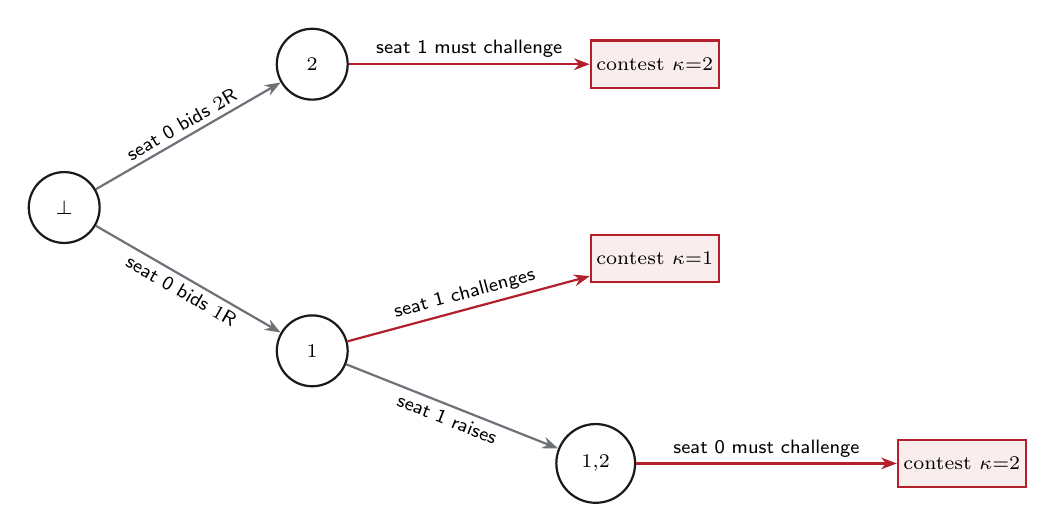
\begin{tikzpicture}[x=15mm,y=-13mm]
  \node[st, minimum size=9mm] (root) at (0,0)     {$\bot$};
  \node[st, minimum size=9mm] (b2)   at (2.1,-1.4){$2$};
  \node[st, minimum size=9mm] (b1)   at (2.1, 1.4){$1$};
  \node[st, minimum size=10mm](b12)  at (4.5, 2.5){$1{,}2$};
  \node[term] (p2)  at (5.0,-1.4) {contest $\kappa{=}2$};
  \node[term] (p1)  at (5.0, 0.5) {contest $\kappa{=}1$};
  \node[term] (p12) at (7.6, 2.5) {contest $\kappa{=}2$};
  \draw[ed]  (root) -- node[lbl,sloped,above=1pt]{seat 0 bids $2\R$} (b2);
  \draw[ed]  (root) -- node[lbl,sloped,below=1pt]{seat 0 bids $1\R$} (b1);
  \draw[ed]  (b1) -- node[lbl,sloped,below=1pt]{seat 1 raises} (b12);
  \draw[edr] (b1) -- node[lbl,sloped,above=1pt]{seat 1 challenges} (p1);
  \draw[edr] (b2) -- node[lbl,above=1pt]{seat 1 must challenge} (p2);
  \draw[edr] (b12) -- node[lbl,above=1pt]{seat 0 must challenge} (p12);
\end{tikzpicture}
\caption{The complete bidding phase of the one-card game, red claims only
(black is the mirror). Node labels are the chain of counts; $\bot$ is the
pre-bid state. Together with the black mirror this is $1+2\cdot 3=7$
states, matching Lemma~\ref{lem:bidcount}.}
\label{fig:h1bid}
\end{figure}

Procurement adds $14$ states and $28$ distinct resolutions
(Table~\ref{tab:round}). A claim of $1$ resolves on the very first flip. A
claim of $2$ admits the three counter pairs $(0,0),(1,0),(0,1)$ before
resolving.

\subsection{Public classes}

With $H=1$, Theorem~\ref{thm:seatcount} gives $K(1)=3$ per-seat statistics
--- $(1,0,0)$, $(1,1,0)$, $(1,0,1)$ --- and Corollary~\ref{cor:classcount}
gives $2\cdot 9+1=19$ classes. Exhaustive forward search
(Section~\ref{sec:reach}) finds $28$ concrete boundary states realizing
$17$ of those $19$.

\begin{example}[The two impossible classes]\label{ex:h1impossible}
The two unreachable classes are $\seat{0}=\seat{1}=(1,0,0)$, for either
loser: a boundary at which \emph{nothing at all} is publicly known about
either card. It cannot occur, because a contest cannot resolve without at
least one flip --- the bidder must either produce a card or bust on one ---
and every flip is public. This is Lemma~\ref{lem:atleastone}.

It is worth noting what is \emph{not} excluded. One might guess that
$\seat{0}=\seat{1}=(1,0,1)$ --- both seats known to hold a black --- is
impossible, on the grounds that under a red claim only one black can ever
be revealed. But the claim need not be red: under a \emph{black} claim of
$2$, the bidder flips one black off each deck, makes the bid, and both
bounds rise together. The class is reachable. Fixing the bid color too
early is the standard way to get these arguments wrong, and we return to it
in Remark~\ref{rem:trap}.
\end{example}

% =========================================================================
\section{Warm-Up II: The Two-Card Game}\label{sec:h2}

Now deal two cards each. Three genuinely new things appear: a bidding
ladder with room to maneuver, a discard that is a real \emph{choice}
rather than a forced elimination, and therefore a second round --- the
first time the game recurses into a smaller copy of itself.

\subsection{Deals and rounds}

There are $\binom{52}{2}\binom{50}{2}=1{,}624{,}350$ card-level deals and
$9$ color outcomes $(r_0,r_1)\in\{0,1,2\}^2$. By
Theorem~\ref{thm:rounds} the game lasts $2$ or $3$ rounds.

\subsection{Structure}

With $T=4$ the opening round has $2^5-1=31$ bidding states, $190$
procurement states and $348$ resolutions. The chain lattice is now
non-trivial: an opener claiming $1$ can be raised to $2$, $3$ or $4$, each
of which can be raised again, and so on.

\begin{figure}[t]
\centering
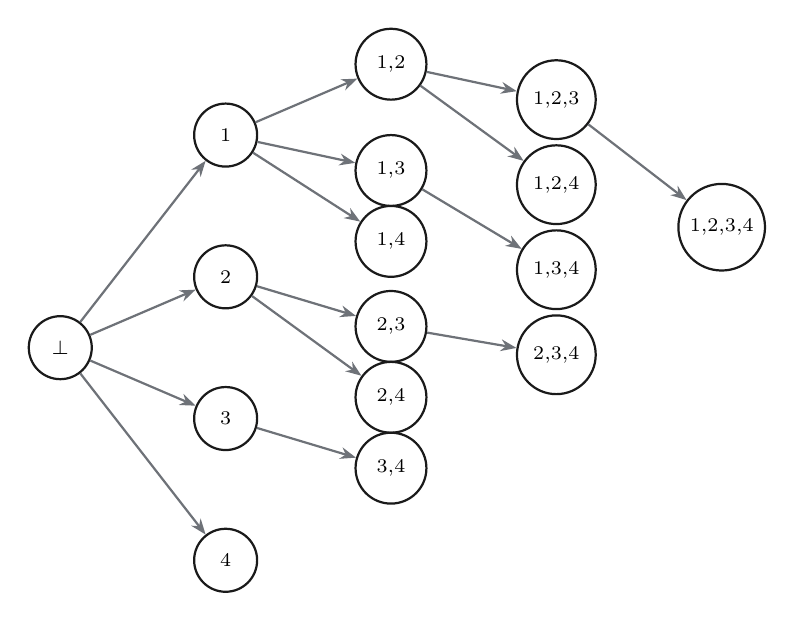
\begin{tikzpicture}[x=21mm,y=-9mm, every node/.style={font=\scriptsize}]
  \node[st,minimum size=8mm] (r) at (0,3.5) {$\bot$};
  \node[st,minimum size=8mm] (a1) at (1,0.5) {$1$};
  \node[st,minimum size=8mm] (a2) at (1,2.5) {$2$};
  \node[st,minimum size=8mm] (a3) at (1,4.5) {$3$};
  \node[st,minimum size=8mm] (a4) at (1,6.5) {$4$};
  \node[st,minimum size=9mm] (b12) at (2,-0.5) {$1{,}2$};
  \node[st,minimum size=9mm] (b13) at (2,1.0) {$1{,}3$};
  \node[st,minimum size=9mm] (b14) at (2,2.0) {$1{,}4$};
  \node[st,minimum size=9mm] (b23) at (2,3.2) {$2{,}3$};
  \node[st,minimum size=9mm] (b24) at (2,4.2) {$2{,}4$};
  \node[st,minimum size=9mm] (b34) at (2,5.2) {$3{,}4$};
  \node[st,minimum size=10mm] (c123) at (3,0.0) {$1{,}2{,}3$};
  \node[st,minimum size=10mm] (c124) at (3,1.2) {$1{,}2{,}4$};
  \node[st,minimum size=10mm] (c134) at (3,2.4) {$1{,}3{,}4$};
  \node[st,minimum size=10mm] (c234) at (3,3.6) {$2{,}3{,}4$};
  \node[st,minimum size=11mm] (d) at (4,1.8) {$1{,}2{,}3{,}4$};
  \foreach \t in {a1,a2,a3,a4} \draw[ed] (r) -- (\t);
  \draw[ed] (a1) -- (b12); \draw[ed] (a1) -- (b13); \draw[ed] (a1) -- (b14);
  \draw[ed] (a2) -- (b23); \draw[ed] (a2) -- (b24);
  \draw[ed] (a3) -- (b34);
  \draw[ed] (b12) -- (c123); \draw[ed] (b12) -- (c124);
  \draw[ed] (b13) -- (c134); \draw[ed] (b23) -- (c234);
  \draw[ed] (c123) -- (d);
\end{tikzpicture}
\caption{The bid-chain lattice for one color at $T=4$: chains are
non-empty subsets of $\{1,2,3,4\}$, so there are $2^4-1=15$ per color and
$2\cdot 15+1=31$ bidding states in total. Every node also has a
\emph{challenge} edge into procurement, omitted here.}
\label{fig:h2ladder}
\end{figure}

\subsection{The first real discard}

At $H=2$ the loser of round~1 holds two cards and must choose which to
drop. This is the game's first genuinely private decision with a future:
the choice is unobserved, it determines the loser's hand for round~2, and
--- by discard anonymity --- the opponent will never learn it directly. It
is also where the public bounds first decay (Lemma~\ref{lem:fold}).

\subsection{Class counts}

$K(2)=9$ per-seat statistics give $2\cdot 81+1=163$ classes, spread over
layers $T=4$ (the root), $T=3$, $T=2$ and $T=1$. Forward search realizes
$149$ of them across $345$ concrete boundary states; the breakdown is in
Table~\ref{tab:reach}.

% =========================================================================
\section{The Full Game}\label{sec:full}

The real game deals $H=5$. There are
\[
  \binom{52}{5}\binom{47}{5} \;=\; 3{,}986{,}646{,}103{,}440
\]
card-level deals and $36$ color outcomes $(r_0,r_1)\in\{0,\dots,5\}^2$,
distributed as in Table~\ref{tab:deallaw}. The opening round alone has
$2{,}047$ bidding states, $65{,}790$ procurement states and $119{,}036$
resolutions.

\begin{table}[t]
\centering
\caption{The color-deal law at $H=5$: $\Pr[r_0=u,\;r_1=v]$, where $r_i$ is
the number of reds dealt to seat $i$. Rows are $u$ (seat $0$), columns $v$
(seat $1$). Mass concentrates on balanced hands, and the slight
anti-diagonal tilt is the without-replacement effect.}
\label{tab:deallaw}
\begin{tabular}{@{}lrrrrrr@{}}
\toprule
& $v=0$ & $1$ & $2$ & $3$ & $4$ & $5$\\
\midrule
$u=0$ & 0.00034 & 0.00257 & 0.00713 & 0.00901 & 0.00518 & 0.00109\\
$1$ & 0.00257 & 0.01783 & 0.04505 & 0.05180 & 0.02713 & 0.00518\\
$2$ & 0.00713 & 0.04505 & 0.10360 & 0.10854 & 0.05180 & 0.00901\\
$3$ & 0.00901 & 0.05180 & 0.10854 & 0.10360 & 0.04505 & 0.00713\\
$4$ & 0.00518 & 0.02713 & 0.05180 & 0.04505 & 0.01783 & 0.00257\\
$5$ & 0.00109 & 0.00518 & 0.00901 & 0.00713 & 0.00257 & 0.00034\\
\bottomrule
\end{tabular}
\end{table}

By Corollary~\ref{cor:classcount} there are $6{,}051$ public classes.
Table~\ref{tab:layers} breaks them down by layer, separating the $330$
terminal classes --- where the pending loser holds one card, so the value
is decided without further play --- from the $5{,}721$ that contain a real
subgame.

\begin{table}[t]
\centering
\caption{Public classes at $H=5$ by layer $T'$ --- the cards in play
\emph{during} the round that follows, i.e.\ after the pending discard
(Definition~\ref{def:layer}).}
\label{tab:layers}
\begin{tabular}{@{}lrrr@{}}
\toprule
$T'$ & With a subgame & Terminal & Total\\
\midrule
$1$  & $0$      & $18$  & $18$\\
$2$  & $36$     & $36$  & $72$\\
$3$  & $132$    & $60$  & $192$\\
$4$  & $330$    & $90$  & $420$\\
$5$  & $686$    & $126$ & $812$\\
$6$  & $1{,}104$  & $0$   & $1{,}104$\\
$7$  & $1{,}290$  & $0$   & $1{,}290$\\
$8$  & $1{,}260$  & $0$   & $1{,}260$\\
$9$  & $882$    & $0$   & $882$\\
$10$ & $1$ (root) & $0$   & $1$\\
\midrule
Total & $5{,}721$ & $330$ & $6{,}051$\\
\bottomrule
\end{tabular}
\end{table}

% =========================================================================
\section{Reachability}\label{sec:reach}

Corollary~\ref{cor:classcount} counts the classes the \emph{definition}
admits. Not all of them can occur. This section characterises the
obstruction, proves it, and reports the exact reachable set.

\subsection{The obstruction}

\begin{lemma}[Every round reveals something]\label{lem:atleastone}
At least one card is flipped in every contest, so at every non-root
boundary at least one of the four bounds is positive.
\end{lemma}

\begin{proof}
The claim's count is at least $1$. The bidder must keep flipping until
either the count is reached --- which requires at least one on-color card
to be revealed --- or an off-color card appears, which is itself a flip.
Either way at least one card is revealed, and by Lemma~\ref{lem:fold} the
corresponding bound is raised to at least $1$.
\end{proof}

\begin{lemma}[Single-round sighting shape]\label{lem:sighting}
Within one round, let $c$ be the bid color. Then the cards revealed from
seat $i$'s deck consist of $m_i\ge 0$ cards of color $c$ together with
$e_i\in\{0,1\}$ cards of the other color, and moreover
$e_0+e_1\le 1$.
\end{lemma}

\begin{proof}
Exactly one color is bid per round. Procurement stops the instant an
off-color card is flipped, so across the whole round at most one
off-color card is ever revealed, and it is the final flip. It comes off
exactly one seat's deck, which gives $e_0+e_1\le 1$ and forces every other
revealed card to be of color $c$.
\end{proof}

\begin{corollary}[One round of history]\label{cor:onernd}
At a boundary reached after exactly one round --- layer $T'=2H-1$, which is
$T'=9$ in the full game --- the bounds satisfy, for some common color $c$:
\begin{enumerate}\itemsep1pt
  \item $\min(\rlb^{\,i},\blb^{\,i})\le 1$ for each seat;
  \item both seats' bounds are expressed against the \emph{same} color
        $c$;
  \item at most one seat has a non-zero bound on the off color.
\end{enumerate}
\end{corollary}

\begin{proof}
Immediate from Lemma~\ref{lem:sighting} and Lemma~\ref{lem:fold}: with only
one round played there is nothing to fold against, so the bounds \emph{are}
the sightings.
\end{proof}

\begin{example}[Three cannot-happen states at $T'=9$]
Corollary~\ref{cor:onernd} rules out, among others:
\begin{center}
\begin{tabular}{@{}lll@{}}
\toprule
Class & Status & Why\\
\midrule
$\seat{0}=(5,3,1)$, $\seat{1}=(5,0,0)$ & reachable & red bid, $3$ reds then a fatal black, all from seat $0$\\
$\seat{0}=(5,2,2)$, $\seat{1}=(5,0,0)$ & impossible & needs two off-color reveals (part 1)\\
$\seat{0}=(5,3,1)$, $\seat{1}=(5,2,1)$ & impossible & needs two off-color reveals (part 3)\\
$\seat{0}=(5,3,0)$, $\seat{1}=(5,0,3)$ & impossible & needs two different bid colors (part 2)\\
\bottomrule
\end{tabular}
\end{center}
\end{example}

\begin{remark}[A trap worth flagging]\label{rem:trap}
Reachability arguments of this kind are easy to get wrong by fixing the bid
color too early. Consider $\ell=0$ with $\seat{0}=(5,1,0)$,
$\seat{1}=(5,0,0)$: seat $0$ owes the discard \emph{and} is known to hold a
red. Reasoning under a red bid, one concludes that no off-color card was
shown, so the bid was made, so exactly one red was produced, so the final
count was $1$; by Remark~\ref{rem:ladder} the bidder was then the starter,
seat $0$, and the loser must therefore be seat $1$ --- contradiction, so
the class looks unreachable. It is not. Under a \emph{black} bid, seat $0$
opens, immediately flips its own top card, and it is red: the contest ends
at once, seat $0$ is the loser, and the revealed red is exactly the
certainty bound. The class is reachable. This is why we compute the closure
by machine rather than argue it by hand.
\end{remark}

Note that the obstruction weakens with depth. After two or more rounds, the
maximum-fold of Lemma~\ref{lem:fold} can combine sightings under
\emph{different} bid colors: a red bid in round~1 revealing $(2,1)$
followed by a black bid in round~2 revealing $(1,2)$ folds to $(2,2)$,
which Corollary~\ref{cor:onernd} forbids after a single round. So the
constraint bites hardest at the top of the game and all but vanishes below.

\subsection{Exact closure}\label{sec:closure}

To decide which classes occur we search the game forward from the deal. But
we cannot search over classes alone, and it is worth being precise about
why.

A class records only what is \emph{certain}: that seat $i$ holds at least
$\rlb^{\,i}$ reds. That is not enough to determine which classes can come
next, because what a seat can \emph{reveal} in the coming round depends on
what it actually holds. A seat whose class says ``at least one red'' might
hold one red or five; only in the latter case can five reds be flipped off
its deck next round, driving $\rlb$ to $5$. So the search must carry the
true hand composition alongside the public bounds.

\begin{definition}[Concrete boundary state]\label{def:concrete}
A \emph{concrete boundary state} is
\[
  \bigl(\ell,\;(r_0,b_0,\rlb^{\,0},\blb^{\,0}),\;
              (r_1,b_1,\rlb^{\,1},\blb^{\,1})\bigr),
\]
where $r_i$ and $b_i$ are the reds and blacks seat $i$ genuinely holds and
the remaining entries are as in Definition~\ref{def:class}. It always
satisfies $\rlb^{\,i}\le r_i$ and $\blb^{\,i}\le b_i$: you cannot be certain
of more than is there.
\end{definition}

Each concrete state determines exactly one class --- forget $r_i$ and $b_i$,
keep $n_i=r_i+b_i$ and the bounds --- so the map
\[
  \{\text{concrete boundary states}\}\;\longrightarrow\;\{\text{classes}\}
\]
is a many-to-one projection, and a class is \emph{reachable} precisely when
at least one concrete state above it is. This is why the two counts in
Table~\ref{tab:reach} differ so much: $27{,}990$ concrete states at $H=5$
collapse onto $5{,}485$ classes, roughly five hands per public description.

\begin{example}
The class $\ell=0$, $s_0=(4,1,0)$, $s_1=(5,0,0)$ says seat $0$ owes a
discard from four cards and certainly holds a red. Sitting above it are the
concrete states with $(r_0,b_0)\in\{(1,3),(2,2),(3,1),(4,0)\}$ --- four
different hands, one public description. Distinguishing them is exactly what
an opponent cannot do.
\end{example}

The search is then a breadth-first closure: start from every color-deal
$(r_0,r_1)$, and from each concrete state generate every state reachable by
one legal round --- every discard the loser could make, every bid color,
every legal final count, either seat as bidder, and every way the contest
could resolve, subject to Lemmas~\ref{lem:atleastone}
and~\ref{lem:sighting}. It terminates because $T$ strictly decreases
(Theorem~\ref{thm:acyclic}) and the state set is finite.

One thing is deliberately \emph{not} carried: how many of a seat's own
discards were red. By Remark~\ref{rem:absent} that changes no legal move and
no public bound, so it cannot affect which classes occur. It does affect
what players believe, which is the subject of the next section.

\begin{table}[t]
\centering
\caption{Exact reachability. ``Enumerable'' counts the classes
Definition~\ref{def:class} admits; ``reachable'' counts those realized by
some deal and some legal play. All three games are closed exhaustively.}
\label{tab:reach}
\begin{tabular}{@{}lrrrr@{}}
\toprule
Game & Boundary states & Reachable classes & Enumerable & Pruned\\
\midrule
$H=1$ & $28$      & $17$      & $19$      & $10.5\%$\\
$H=2$ & $345$     & $149$     & $163$     & $8.6\%$\\
$H=5$ & $27{,}990$ & $5{,}485$ & $6{,}051$ & $9.4\%$\\
\bottomrule
\end{tabular}

\vspace{9pt}

\begin{tabular}{@{}lrrr@{}}
\toprule
$H=5$, layer $T'$ & Reachable & Enumerable & Pruned\\
\midrule
$1$  & $16$      & $18$      & $11.1\%$\\
$2$  & $68$      & $72$      & $5.6\%$\\
$3$  & $186$     & $192$     & $3.1\%$\\
$4$  & $412$     & $420$     & $1.9\%$\\
$5$  & $802$     & $812$     & $1.2\%$\\
$6$  & $1{,}096$ & $1{,}104$ & $0.7\%$\\
$7$  & $1{,}284$ & $1{,}290$ & $0.5\%$\\
$8$  & $1{,}256$ & $1{,}260$ & $0.3\%$\\
$9$  & $364$     & $882$     & $\mathbf{58.7\%}$\\
$10$ & $1$       & $1$       & $0\%$\\
\midrule
Total & $5{,}485$ & $6{,}051$ & $9.4\%$\\
\bottomrule
\end{tabular}
\end{table}

\begin{figure}[t]
\centering
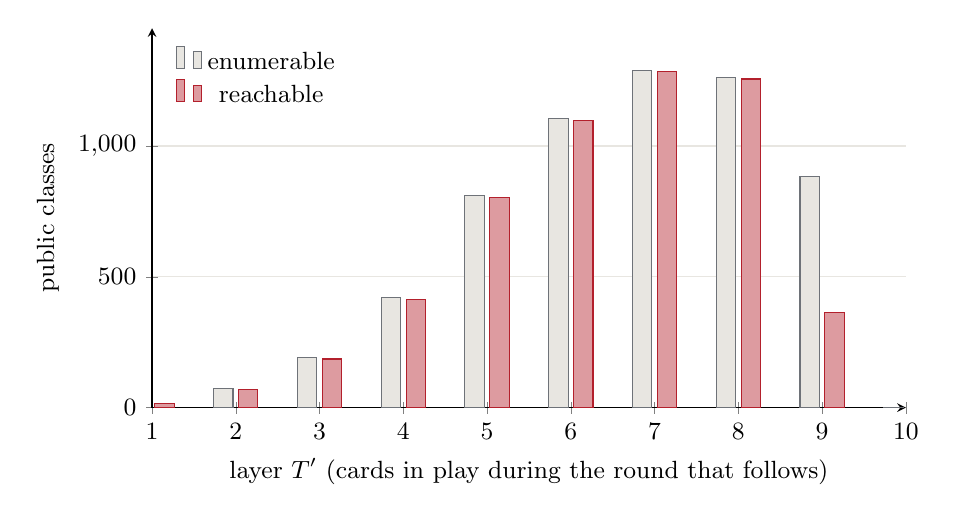
\begin{tikzpicture}
\begin{axis}[
  width=0.92\textwidth, height=6.4cm,
  ybar, bar width=7pt,
  xlabel={layer $T'$ (cards in play during the round that follows)},
  ylabel={public classes},
  xtick=data, symbolic x coords={1,2,3,4,5,6,7,8,9,10},
  ymin=0, ymax=1450,
  legend style={at={(0.02,0.97)}, anchor=north west, draw=none,
                fill=white, font=\small},
  tick label style={font=\small}, label style={font=\small},
  axis lines=left, ymajorgrids, grid style={draw=rblight},
]
\addplot[draw=rbgrey, fill=rblight] coordinates
  {(1,18) (2,72) (3,192) (4,420) (5,812) (6,1104) (7,1290) (8,1260) (9,882) (10,1)};
\addplot[draw=rbred, fill=rbred!45] coordinates
  {(1,16) (2,68) (3,186) (4,412) (5,802) (6,1096) (7,1284) (8,1256) (9,364) (10,1)};
\legend{enumerable, reachable}
\end{axis}
\end{tikzpicture}
\caption{Enumerable versus reachable public classes by layer. The two
series are nearly identical everywhere except $T'=9$ --- the layer reached
after exactly one round, where Corollary~\ref{cor:onernd} eliminates
$58.7\%$ of the classes the definition admits.}
\label{fig:reachplot}
\end{figure}

\subsection{Reading the result}

Two things stand out. First, the reachable set is $90.6\%$ of the
enumerable one, so the definition of a public class is tight: the
statistics in Definition~\ref{def:class} are very nearly a complete
invariant. Second, essentially all of the slack sits in a single layer.
$T'=9$ is the only layer with exactly one round of history, and
Corollary~\ref{cor:onernd} is strongest there; by $T'=8$ two rounds of
max-folding have already restored almost everything.

\begin{figure}[t]
\centering
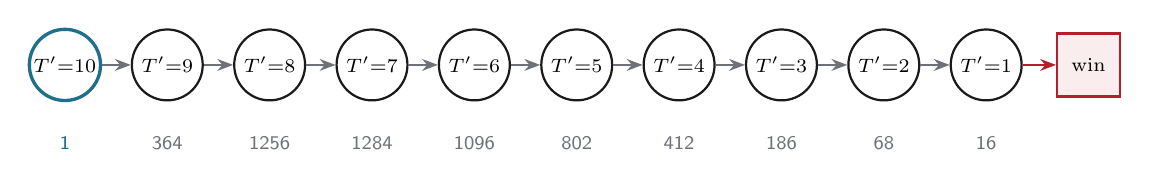
\begin{tikzpicture}[x=13mm,y=-11mm, every node/.style={font=\scriptsize}]
  \node[st,minimum size=9mm,draw=rbaccent,very thick] (t10) at (0,0) {$T'{=}10$};
  \foreach \i/\lab in {1/9,2/8,3/7,4/6,5/5,6/4,7/3,8/2,9/1}{
    \node[st,minimum size=9mm] (t\lab) at (\i,0) {$T'{=}\lab$};
  }
  \node[term,minimum size=8mm] (end) at (10,0) {win};
  \foreach \a/\b in {t10/t9, t9/t8, t8/t7, t7/t6, t6/t5, t5/t4, t4/t3, t3/t2, t2/t1}{
    \draw[ed] (\a) -- (\b);
  }
  \draw[edr] (t1) -- (end);
  \foreach \lab/\n in {9/364, 8/1256, 7/1284, 6/1096, 5/802, 4/412, 3/186, 2/68, 1/16}{
    \node[lbl, text=rbgrey] at ($(t\lab)+(0,0.9)$) {\n};
  }
  \node[lbl, text=rbaccent] at ($(t10)+(0,0.9)$) {1};
\end{tikzpicture}
\caption{The layered class DAG of the full game. Play enters at the unique
root and descends exactly one layer per round, since every round removes
exactly one card; the game therefore terminates after between $5$ and $9$
rounds (Theorem~\ref{thm:rounds}). Figures beneath each node are the
reachable class counts of Table~\ref{tab:reach}.}
\label{fig:layerdag}
\end{figure}

% =========================================================================
\section{What the Public Class Forgets}\label{sec:forgets}

The public class of Definition~\ref{def:class} is a summary, and summaries
discard things. This section says exactly what it discards, because the
omissions are not incidental --- they are the reason the companion paper's
decomposition needs care.

\subsection{Knowledge versus belief}

There is a sharp answer to what the class keeps.

\begin{theorem}[Support completeness]\label{thm:support}
Fix a reachable class $(\ell,s_0,s_1)$. The hand compositions consistent
with \emph{some} history reaching it are exactly
\[
  \bigl\{(r_i,b_i)\;:\;r_i\ge \rlb^{\,i},\;\; b_i\ge \blb^{\,i},\;\;
                        r_i+b_i=n_i,\;\; i=0,1\bigr\}.
\]
That is, the certainty bounds are simultaneously \emph{sound} (nothing
outside the box is possible) and \emph{tight} (everything inside it occurs).
\end{theorem}

\noindent Soundness is Lemma~\ref{lem:fold}. Tightness is verified
exhaustively: across all $5{,}485$ reachable classes at $H=5$, the hand
compositions actually realized by the closure of Section~\ref{sec:closure}
fill the box exactly, with no class showing a gap.

So the class is a \emph{complete} record of what is publicly \textbf{known}.
It is not a record of what is publicly \textbf{believed}. Knowing the
support of a distribution is not knowing the distribution, and the gap
between the two is large enough to matter.

\subsection{Two paths to the same class}

Consider a seat that ends up holding four cards, certainly including at
least one red --- public statistic $(4,1,0)$. Two histories reach it:

\begin{description}\itemsep3pt
  \item[Path A (decay).] The seat held five cards; \emph{two reds were
        flipped off its deck} in round~1. It lost, and discarded. The bound
        rose to $2$, then decayed by one: $\rlb=1$, $n=4$.
  \item[Path B (fresh sighting).] The seat held five cards and nothing was
        revealed from it in round~1. It lost and discarded, leaving four
        cards and no bounds. In round~2 \emph{one red} was flipped off its
        deck: $\rlb=1$, $n=4$.
\end{description}

Identical classes. But an observer who watched Path A saw two reds go into
that hand and only one card leave it, so it very likely still holds two.
An observer of Path B saw one red and nothing else. Table~\ref{tab:paths}
quantifies the gap under a neutral reference policy --- uniformly random
ordering and uniformly random discard --- chosen only to put numbers on it.

\begin{table}[htbp]
\centering
\caption{Posterior over the reds a seat holds, given the \emph{same} public
statistic $(n,\rlb,\blb)=(4,1,0)$. Both paths certify ``at least one red''
and neither certifies more --- the bound is tight for each --- yet the
distributions differ substantially.}
\label{tab:paths}
\begin{tabular}{@{}lrr@{}}
\toprule
Reds held & Path A (two seen, then discard) & Path B (discard, then one seen)\\
\midrule
$1$ & $0.0531$ & $0.1248$\\
$2$ & $0.3184$ & $0.3902$\\
$3$ & $0.4521$ & $0.3745$\\
$4$ & $0.1765$ & $0.1104$\\
\midrule
Expected reds        & $2.752$ & $2.471$\\
$\Pr[\text{at least }2\text{ reds}]$ & $0.947$ & $0.875$\\
\bottomrule
\end{tabular}
\end{table}

The mechanism is the max-fold of Lemma~\ref{lem:fold}. Folding is
\emph{lossy in a specific direction}: it remembers the height of the bound
but forgets whether that height is fresh evidence or the residue of a taller
bound worn down by discards. A bound of $1$ that used to be $3$ is a much
stronger signal than a bound of $1$ that has always been $1$, and the class
cannot tell them apart.

\subsection{The bid history}

The second omission is blunter: a round's bid history is cleared when the
round ends (Section~\ref{sec:info}) and appears nowhere in the class. Yet
bids are chosen by players who can see their own cards, so a bid history is
evidence about the bidder's hand, and a \emph{sequence} of bid histories is
evidence about how that player bids --- how readily they bluff, how they
price a raise.

Neither kind of evidence survives into the public class. Note the
asymmetry with the flip record: flips are physical reveals and enter the
class as bounds; bids are cheap talk and enter not at all. A player who
opened $5\R$ last round and was caught has told the table something real,
and the class forgets it completely.

\subsection{Why the class stops where it does}

It would be natural to ask for a finer public state, and worth seeing why
one is not simply available.

The exact public posterior over hands depends on the players'
\emph{strategies}. If I know you always discard a black when you hold one,
watching you discard is enormously informative; if I know nothing about your
policy, the same observation tells me almost nothing. So the exact posterior
is not a function of the public history alone --- it is a function of the
history \emph{and} a model of the opponent. It cannot be tabulated as part
of a description of the game, because it is not a property of the game.

The certainty bounds are what remains once that dependence is stripped out.
They are precisely the facts entailed by the rules and the public record
regardless of how anyone has been playing, which is why they, and not some
richer statistic, are the right stopping point for a paper about the game
itself. Theorem~\ref{thm:support} is the formal version of that claim: the
class is exactly the strategy-independent content of the public history.

Everything beyond it --- the fold's path dependence, the bid history, the
opponent's discard tendencies --- is belief rather than knowledge, and
belongs to a paper that commits to a strategy model. That is the next one.

\section{Summary of Counts}\label{sec:summary}

Table~\ref{tab:master} gathers every quantity derived above across the
three games. Reading it left to right shows how sharply the game grows with
hand size: the deal count climbs by nine orders of magnitude, and the
opening round's contest structure by four, while the \emph{public} state
space --- the thing an observer must actually track --- grows only from
$19$ to $6{,}051$. That gap is the point of Section~\ref{sec:public}: the
public projection is exponentially smaller than the machine it summarizes,
and it is what the companion paper's algorithms index on.

\begin{table}[!ht]
\centering
\caption{Master table. Every entry is produced by \code{state\_counts.py}
and, where an engine counterpart exists, verified against the shipped
implementation by \code{verify\_against\_engine.py}.}
\label{tab:master}
\begin{tabular}{@{}lrrr@{}}
\toprule
Quantity & $H=1$ & $H=2$ & $H=5$\\
\midrule
Card-level deals            & $2{,}652$ & $1{,}624{,}350$ & $3{,}986{,}646{,}103{,}440$\\
Color-level deal outcomes  & $4$ & $9$ & $36$\\
Rounds (min--max)           & $1$--$1$ & $2$--$3$ & $5$--$9$\\
Opening-round bid states    & $7$ & $31$ & $2{,}047$\\
Opening-round procurement   & $14$ & $190$ & $65{,}790$\\
Opening-round resolutions   & $28$ & $348$ & $119{,}036$\\
Per-seat public statistic $K(H)$ & $3$ & $9$ & $55$\\
Public classes $2K^2+1$     & $19$ & $163$ & $6{,}051$\\
\quad of which terminal     & $18$ & $54$ & $330$\\
\quad of which reachable    & $17$ & $149$ & $5{,}485$\\
Concrete boundary states    & $28$ & $345$ & $27{,}990$\\
\bottomrule
\end{tabular}
\end{table}

\section{What Comes Next}\label{sec:next}

This paper deliberately stops at the dynamics. Three threads carry into the
companion paper on counterfactual regret minimization.

\paragraph{From public classes to information sets.} A player at a boundary
knows their public class \emph{and} their own hand. The private component
turns out to need two numbers, not one: the reds currently held, and the
reds among the cards that player has itself discarded. The second is
private information about the \emph{deck}, not about the hand --- which
brings us to the next thread.

\paragraph{The finite deck is load-bearing.} Because the deck is finite and
balanced, your own cards tell you about your opponent's. Seeing $k$ reds
among your own five shifts the chance an unseen card is red from $1/2$ to
$(26-k)/47$, a swing from $0.447$ to $0.553$. In the one-card game this is
the \emph{entire} strategic content: the opener's only real decision is
whether to bet that the two cards match or differ, and it should use its
own five dealt cards to choose. That game's exact value is
$\tfrac{40651}{78302}\approx 0.5192$ to the opener --- above $1/2$ purely
because of sampling without replacement, and above the $26/51\approx0.5098$
that an opener ignoring its own cards would get. Under an idealised
infinite deck the same game is exactly even.

\paragraph{Composition is the hard part.} The layered DAG of
Section~\ref{sec:reach} invites solving the game layer by layer,
bootstrapping each class from the ones below. Two hazards, both visible
from this paper, make that harder than it looks. First, by
Section~\ref{sec:forgets} the class is not a sufficient statistic for
beliefs, so re-deriving a belief from the class at a layer boundary is an
approximation, not an identity --- it silently merges the two paths of
Table~\ref{tab:paths}. Second, whether the decomposition is faithful
depends on where the layers are cut relative to the private discard
decision. Getting either wrong is not a small error. Both are the subject
of the companion paper.

\appendix

\section{Reproducing the numbers}\label{app:repro}

Two scripts accompany this paper.

\begin{description}\itemsep3pt
  \item[\code{state\_counts.py}] re-derives every count from the rules,
        independently of the game engine, and prints all tables in this
        paper. It includes the forward-closure search of
        Section~\ref{sec:reach}.
  \item[\code{verify\_against\_engine.py}] cross-checks the round-automaton
        counts, the class-space counts and the reachable set against the
        shipped implementation, so any disagreement is a genuine bug in one
        of the two rather than a difference of convention.
\end{description}

\noindent Run them with
\begin{quote}
\code{cd research \&\& ../simulator/.venv/bin/python state\_counts.py}\\
\code{cd research \&\& ../simulator/.venv/bin/python verify\_against\_engine.py}
\end{quote}

\section{Glossary}

\begin{description}\itemsep2pt
  \item[Boundary] The moment a contest resolves: loser known, discard not
        yet made. The natural cut point for describing the public state.
  \item[Chain] The strictly increasing sequence of counts bid in a round.
  \item[Class] The public state at a boundary
        (Definition~\ref{def:class}).
  \item[Layer $T$] Total cards in play after the pending discard; strictly
        decreasing, hence a valid induction index.
  \item[Procurement] The contest phase: the bidder flips cards trying to
        produce the claim.
  \item[Sighting] The multiset of colors revealed from one seat's deck in
        one round.
\end{description}

\end{document}
